\documentclass[aspectratio=169,10pt]{beamer}
\usetheme{default}
\usecolortheme{seahorse}
\setbeamertemplate{navigation symbols}{}
\setbeamertemplate{footline}[frame number]
\setbeamertemplate{itemize items}[circle]
\setbeamerfont{frametitle}{size=\normalsize,series=\bfseries}
\setbeamercolor{frametitle}{fg=blue!50!black}
\usepackage{booktabs}
\usepackage{xcolor}
\usepackage{graphicx}
\usepackage{array}
\usepackage{tikz}
\usetikzlibrary{arrows.meta,positioning,fit}
\newcommand{\fitw}[1]{\resizebox{\linewidth}{!}{#1}}
\newcommand{\code}[1]{\texttt{#1}}
\newcommand{\good}[1]{{\color{green!45!black}\textbf{#1}}}
\newcommand{\bad}[1]{{\color{red!70!black}\textbf{#1}}}
\newcommand{\gh}{https://github.com/HaiwangYu/fm4npp-lartpc}
\newcommand{\iss}[1]{\href{\gh/issues/#1}{\color{blue!60!black}\##1}}
\newcommand{\doc}[1]{\href{\gh/blob/main/multi-modal-qlmatch/docs/#1}{\color{blue!60!black}\texttt{#1}}}
\setlength{\tabcolsep}{4pt}
\tikzset{box/.style={draw=blue!40!black, rounded corners=2pt, fill=blue!4, align=center, font=\scriptsize,
                     inner sep=3pt, minimum height=0.9cm},
         note/.style={align=left, font=\tiny, text=black!70},
         arr/.style={-{Stealth[length=4pt]}, thick, blue!40!black}}

\title{SBND real data with Wire-Cell labels}
\subtitle{What is in the samples, how Wire-Cell labels them, and the first qlfm tests}
\author{Haiwang Yu}
\institute{fm4npp-lartpc \;\textbullet\; issue \iss{14} (data), \iss{11} (simulation)}
\date{22 November 2026}

\begin{document}

\begin{frame}
  \titlepage
  \vfill
  {\tiny All numbers from the converted samples on Polaris and the reports in \code{\$QLFM\_WORK/sbnd\_data/}.
  Prepared with the assistance of Claude (Anthropic).}
\end{frame}

%=====================================================================
\begin{frame}{Summary}
  \footnotesize
  \begin{itemize}\setlength{\itemsep}{5pt}
    \item \textbf{Data:} 89,946 beam-on events (open SBND run-1 BNB data, 4.62e18 POT) and 49,970 off-beam events, both
      light-triggered, converted to the same HDF5 layout as the 923k-event SBND simulation. Real data has no truth; the
      reference label is Wire-Cell's.
    \item \textbf{Wire-Cell label:} a hit is ``$\nu$'' if it lies on the 2D footprint of a Wire-Cell $\nu$ candidate: a
      cluster matched to a beam-window flash, after the through-going, stopping-muon and light-mismatch vetoes. Same
      Wire-Cell release (WCT 0.38.0) on data and simulation. On simulation it has efficiency 0.92 and purity 0.95.
    \item \textbf{Data vs simulation (first look):} data hits are narrower on V ($-3\%$) and Y ($-4.5\%$), the same at
      every drift distance; more low-charge hits; beam-on light about 0.3\,$\mu$s later.
    \item \textbf{13 simulation-trained qlfm models on real data:}
      \begin{itemize}
        \item hit level: agreement with Wire-Cell falls from $\approx$0.9 on simulation to \bad{0.5--0.65} on beam-on;
        \item event level: at Wire-Cell's off-beam rate they select 31--32\% of beam-on events, Wire-Cell 45\%;
        \item fine-tuned pretrained models are best; frozen and no-pretraining models are clearly worse.
      \end{itemize}
    \item \textbf{Same simulation-to-data gap as on MicroBooNE} (\iss{10}). Its cause on SBND is not tested yet.
  \end{itemize}
\end{frame}

%=====================================================================
\begin{frame}{The campaign: steps and who did them}
  \footnotesize
  \centering
  \fitw{\begin{tabular}{llll}
    \toprule
    date (2026) & step & by & record \\
    \midrule
    Nov 20 & recipe; \code{sbnd-h5maker} 0.5 \code{--data} mode, tested on 67 selected events & prod\_aurora (Aurora) & \doc{sbnd-realdata.md} \\
    Nov 20 & owner choices: open run-1 BNB data, InTime-Run1 off-beam, Wire-Cell option B (WCT 0.38.0) & Haiwang & \iss{14} \\
    Nov 20 & 10-event test files; review: layout, labels, light timing OK & porting\_sbndbuild03 / fmlar\_polaris & \iss{14} \\
    Nov 21 & full production on FermiGrid: 288 jobs, 37.5 CPU-h; copied to Eagle, sha256 verified & porting\_sbndbuild03 & \iss{14} \\
    Nov 21 & simulation rebuilt with the same Wire-Cell (0.38.0) labels & prod\_aurora & \iss{14} \\
    Nov 22 & conversion to the qlfm cache (1 node, 2 min); first look vs simulation (E3) & fmlar\_polaris (Polaris) & \iss{14} \\
    Nov 22 & 13 models vs Wire-Cell on beam-on / off-beam (E4) & fmlar\_polaris & \iss{14} \\
    \bottomrule
  \end{tabular}}\\[6pt]
  \raggedright\scriptsize
  The three agents are Claude Code sessions working for Haiwang: \code{prod\_aurora} (ALCF Aurora), \code{porting\_sbndbuild03} (FNAL),
  \code{fmlar\_polaris} (ALCF Polaris). Owner decisions are Haiwang's.
\end{frame}

%=====================================================================
\section{What is in the data}
\begin{frame}{Samples}
  \footnotesize
  \centering
  \fitw{\begin{tabular}{lllll}
    \toprule
    & \textbf{beam-on} & \textbf{off-beam} & \textbf{simulation (reference)} \\
    \midrule
    source & open FixedDev BNB data, run 1 & InTime-Run1 off-beam & Gen2 MC (BNB CV, $\nu_e$CC, NC $\Delta$-rad) \\
    reco1 & MCP2025C Fall25, v10\_14\_02 & SBND2026A gen2, v10\_14\_02\_02 & v10\_14\_02\_03, CORSIKA cosmics \\
    runs & 18255, 18259 & InTime run 1 & -- \\
    DAQ stream & \code{bnblight} (BNB gate + light) & \code{offbeamlight} (off-beam gate + light) & no trigger emulation \\
    filter & DigitalNoiseEventFilter & DigitalNoiseEventFilter & -- \\
    files / events & 1,817 / \textbf{89,946} & 1,058 / \textbf{49,970} & 1,781 / \textbf{922,788} \\
    exposure & 4.62e18 POT (from CAFs) & no spill count & -- \\
    size (HDF5) & 26.3 GB & 15.0 GB & 349 GB \\
    hits & 1,160.6M & 664.8M & -- \\
    \bottomrule
  \end{tabular}}\\[6pt]
  \raggedright\scriptsize
  \begin{itemize}
    \item The blinded \code{SBND2026A gen2\_BNB-Run1} data set is never used.
    \item Both data samples are \textbf{light-triggered}: rates below are per light-triggered event, not per spill. The
      simulation has a neutrino in every BNB CV event and no trigger selection.
    \item Files: Eagle \code{fm4npp-lartpc-data/sbnd-data-\{bnb-opendata,offbeam-intime-run1\}/}, each with
      \code{full/}, \code{lists/} and a README.
  \end{itemize}
\end{frame}

\begin{frame}{Production chain}
  \centering
  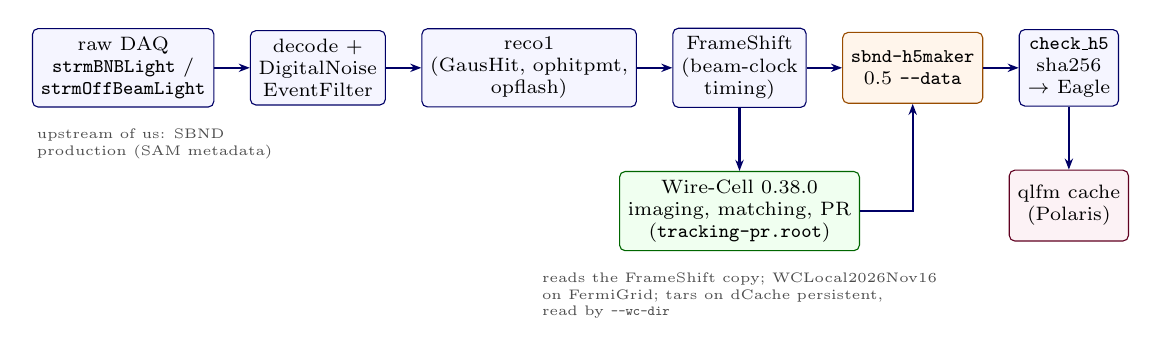
\begin{tikzpicture}[node distance=0.35cm and 0.45cm]
    \node[box] (raw) {raw DAQ\\\code{strmBNBLight} /\\\code{strmOffBeamLight}};
    \node[box, right=of raw] (dec) {decode +\\DigitalNoise\\EventFilter};
    \node[box, right=of dec] (reco) {reco1\\(GausHit, ophitpmt,\\opflash)};
    \node[box, right=of reco] (fs) {FrameShift\\(beam-clock\\timing)};
    \node[box, right=of fs, fill=orange!8, draw=orange!60!black] (h5) {\code{sbnd-h5maker}\\0.5 \code{--data}};
    \node[box, below=0.8cm of fs, fill=green!6, draw=green!40!black] (wc) {Wire-Cell 0.38.0\\imaging, matching, PR\\(\code{tracking-pr.root})};
    \node[box, right=of h5] (chk) {\code{check\_h5}\\sha256\\$\to$ Eagle};
    \node[box, below=0.8cm of chk, fill=purple!5, draw=purple!50!black] (q) {qlfm cache\\(Polaris)};
    \draw[arr] (raw) -- (dec); \draw[arr] (dec) -- (reco); \draw[arr] (reco) -- (fs); \draw[arr] (fs) -- (h5);
    \draw[arr] (h5) -- (chk); \draw[arr] (chk) -- (q);
    \draw[arr] (fs.south) -- (wc.north); \draw[arr] (wc.east) -| (h5.south);
    \node[note, below=0.15cm of wc] {reads the FrameShift copy; WCLocal2026Nov16\\on FermiGrid; tars on dCache persistent,\\read by \code{--wc-dir}};
    \node[note, below=0.15cm of raw, xshift=0.4cm] {upstream of us: SBND\\production (SAM metadata)};
  \end{tikzpicture}\\[8pt]
  \raggedright\scriptsize
  \begin{itemize}\setlength{\itemsep}{2pt}
    \item \textbf{Per reco1 file} (``pair'') on FermiGrid: copy, FrameShift, untar the Wire-Cell output, run \code{sbnd\_h5maker.py --data},
      run \code{check\_h5.py}. 288 jobs of 10 pairs, about 1.5 h elapsed (cluster 30819860).
    \item \textbf{FrameShift} supplies \code{frame\_apply\_at\_caf\_ns} (0.25--2.8\,$\mu$s): light times move from the trigger
      clock to the beam clock, $t_\mathrm{beam} = t_\mathrm{peak} + \code{frame\_apply\_at\_caf\_ns}/1000$, as Wire-Cell does.
    \item The simulation went through the same \code{sbnd-h5maker} (0.4) and the same Wire-Cell 0.38.0 step (rebuilt 21 Nov).
  \end{itemize}
\end{frame}

\begin{frame}{What one HDF5 file holds (same layout as the simulation)}
  \footnotesize
  \centering
  \fitw{\begin{tabular}{lp{7.3cm}p{4.6cm}}
    \toprule
    table & content (one row per \dots) & data vs simulation \\
    \midrule
    \code{event\_table} & event: run/subrun/event, beam gate, time, FrameShift timing, Wire-Cell status and bundle census
      (\code{wc\_n\_bundle}, \code{wc\_n\_bundle\_cosmic}) & data: truth columns at defaults ($\nu$ PDG 0, vertex $-9999$) \\
    \code{hit\_table} & GausHit: channel, TPC, plane, wire, peak time, RMS, integral, amplitude & same producer label (\code{gaushit}) \\
    \code{ophit\_table} & PMT optical hit (\code{ophitpmt}): channel, peak time, width, area, PE; window $-10\dots40\,\mu$s & times on the trigger clock in the file \\
    \code{opflash\_table}, \code{opflashsumpe\_table} & flashes (\code{opflashtpc0/1}) and their per-PMT PE & -- \\
    \code{wc\_event\_table} & Wire-Cell $\nu$ candidate: cluster, flash time / PE / TPC, reco vertex and energy, $\nu_\mu$/$\nu_e$ scores,
      containment, \code{cosmict\_flag} & \code{cosmict\_flag} new in 0.5 \\
    \code{wc\_hit\_table} & per hit (same order as \code{hit\_table}): Wire-Cell cluster id, $\nu$-candidate index, main cluster & the label \\
    \code{nu\_table}, \code{edep\_table}, \code{particle\_table} & truth: neutrinos, Geant4 deposits projected onto hits, particles & \textbf{empty in data} \\
    \bottomrule
  \end{tabular}}\\[6pt]
  \raggedright\scriptsize
  File attributes record the detector, units, the producer labels, the Wire-Cell channel and tick conventions, and the label
  definition (\code{wc\_label\_notes}). Data: \code{is\_data} = 1, no \code{sim\_config}.
\end{frame}

\begin{frame}{Hits and light: same producers, different upstream chains}
  \footnotesize
  \begin{columns}[T]
    \begin{column}{0.58\textwidth}
      \centering
      \scriptsize
      \fitw{\begin{tabular}{lll}
        \toprule
        & simulation & real data \\
        \midrule
        reco1 release & sbndcode v10\_14\_02\_03 & production MCP2025C (v10\_14\_02) \\
        waveforms into GausHit & Wire-Cell 2D sim + noise filter + SP & noise filter + SP on real waveforms \\
        field response & \code{garfield-sbnd-v1} & the detector \\
        noise & spectra scaled from ProtoDUNE-SP & the detector \\
        hit finder & \code{gaushit} (\code{sbnd\_gaushitfinder}) & \code{gaushit} \\
        light & semi-analytic photon sim, \code{opdaq} & 120 PMTs \\
        diffusion ($D_L$, $D_T$) & 4.0, 8.8 cm$^2$/s & -- \\
        \bottomrule
      \end{tabular}}
    \end{column}
    \begin{column}{0.40\textwidth}
      \begin{itemize}\setlength{\itemsep}{3pt}
        \item The HDF5 records only the producer label for data. That the data GausHit settings equal the simulation's is
          \textbf{not verified} (the FHiCL of one data reco1 file would settle it).
        \item Geometry: 2 TPCs (drift $\pm$200\,cm), 3 planes each (U, V induction; Y collection), 0.3\,cm pitch, 0.5\,$\mu$s ticks.
        \item qlfm mirrors TPC 1 onto one drift axis and keys tokens on the TPC; light enters as 120 PMT tokens, 16 time bins.
      \end{itemize}
    \end{column}
  \end{columns}
\end{frame}

\begin{frame}{What qlfm reads (converted cache on Polaris)}
  \footnotesize
  \begin{columns}[T]
    \begin{column}{0.52\textwidth}
      \begin{itemize}\setlength{\itemsep}{3pt}
        \item \textbf{Inputs:} per hit plane, wire, drift tick, TPC, integral, RMS; per optical hit PMT, time (beam clock), PE.
        \item \textbf{Labels / references} (never model input):
          \begin{itemize}
            \item \code{hit\_pnd\_nu}: Wire-Cell $\nu$-candidate footprint;
            \item \code{hit\_pnd\_nu\_ct0}: the same, candidates passing the PR cosmic tagger;
            \item per event: brightest flash time and PE, run/subrun/event.
          \end{itemize}
        \item \textbf{Conversion:} \code{QLFM\_DETECTOR=sbnd}, 2,875 files in 2 min on one node, exit 0 for all; merged into
          61 + 36 shards; first and last shard checked column by column against their sources.
      \end{itemize}
    \end{column}
    \begin{column}{0.46\textwidth}
      \centering
      \scriptsize
      \begin{tabular}{lrr}
        \toprule
        & beam-on & off-beam \\
        \midrule
        events & 89,946 & 49,970 \\
        hits & 1,160.6M & 664.8M \\
        optical hits & 181.0M & 105.4M \\
        hits / event & 12.9k & 13.3k \\
        shards & 61 & 36 \\
        \bottomrule
      \end{tabular}\\[4pt]
      {\tiny Cache: \code{\$QLFM\_WORK/cache/sbnd\_data\_m/}. Simulation cache: \code{cache/sbnd\_m/} (12.4k hits / event).}
    \end{column}
  \end{columns}
\end{frame}

%=====================================================================
\section{How Wire-Cell labels}
\begin{frame}{Wire-Cell: from charge and light to a $\nu$ candidate}
  \centering
  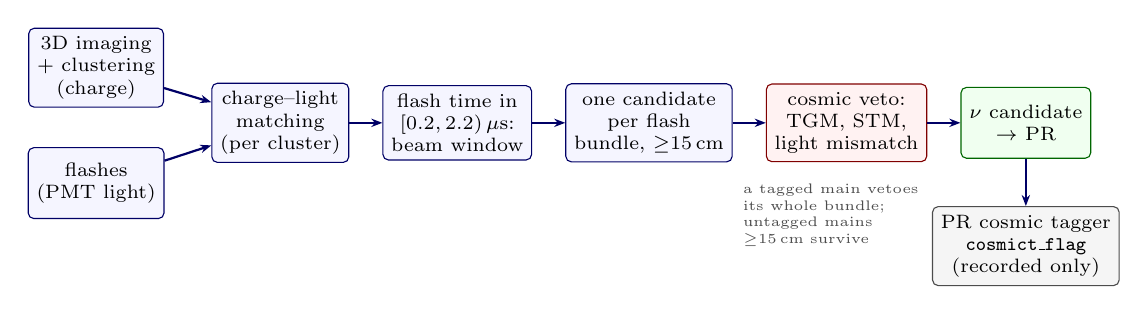
\begin{tikzpicture}[node distance=0.3cm and 0.42cm]
    \node[box] (img) {3D imaging\\+ clustering\\(charge)};
    \node[box, below=0.5cm of img] (fl) {flashes\\(PMT light)};
    \node[box, right=0.6cm of img, yshift=-0.7cm] (m) {charge--light\\matching\\(per cluster)};
    \node[box, right=of m] (bw) {flash time in\\$[0.2, 2.2)\,\mu$s:\\beam window};
    \node[box, right=of bw] (b) {one candidate\\per flash\\bundle, $\ge$15\,cm};
    \node[box, right=of b, fill=red!5, draw=red!50!black] (veto) {cosmic veto:\\TGM, STM,\\light mismatch};
    \node[box, right=of veto, fill=green!6, draw=green!40!black] (nu) {$\nu$ candidate\\$\to$ PR};
    \node[box, below=0.6cm of nu, fill=gray!8, draw=gray!60!black] (ct) {PR cosmic tagger\\\code{cosmict\_flag}\\(recorded only)};
    \draw[arr] (img) -- (m); \draw[arr] (fl) -- (m); \draw[arr] (m) -- (bw); \draw[arr] (bw) -- (b); \draw[arr] (b) -- (veto);
    \draw[arr] (veto) -- (nu); \draw[arr] (nu) -- (ct);
    \node[note, below=0.15cm of veto, xshift=-0.2cm] {a tagged main vetoes\\its whole bundle;\\untagged mains\\$\ge$15\,cm survive};
  \end{tikzpicture}\\[8pt]
  \raggedright\scriptsize
  \begin{itemize}\setlength{\itemsep}{2pt}
    \item Code: \code{clus.jsonnet}, \code{TaggerCheckNeutrino} (\code{nu\_per\_bundle}, \code{nu\_skip\_cosmic}, \code{nu\_skip\_cosmic\_bundle}).
      The same in the earlier aurora-r2 and in 0.38.0.
    \item TGM = through-going muon, STM = stopping muon; ``light mismatch'' = the cluster's predicted light disagrees with the matched flash.
    \item The PR-level cosmic tagger (OR of ten tests, plus a BDT score) and the $\nu_\mu$/$\nu_e$ scores are stored per candidate,
      \textbf{not applied} to the label. Note: \code{cosmic\_flag} is a BDT input, not the verdict.
  \end{itemize}
\end{frame}

\begin{frame}{From a candidate to a per-hit label}
  \footnotesize
  \begin{columns}[T]
    \begin{column}{0.54\textwidth}
      \begin{enumerate}\setlength{\itemsep}{4pt}
        \item \textbf{Footprint:} for every cluster of every candidate, Wire-Cell's 2D projection (\code{T\_proj\_data}): a list of
          (channel, 4-tick time slice) cells.
        \item \textbf{Match each GausHit} to a cell by channel and slice $\lfloor(t_\mathrm{peak} + 0)/4\rfloor$.
          Channels are first mapped to Wire-Cell's numbering:
          \begin{itemize}
            \item Wire-Cell: plane-major, [U0 U1][V0 V1][Y0 Y1];
            \item LArSoft: TPC-major, [U0 V0 Y0][U1 V1 Y1];
            \item offsets $(0, +1984, +3968)$ for TPC 0, $(-3654, -1670, 0)$ for TPC 1.
          \end{itemize}
        \item \textbf{Labels:} \code{wc} = hit on any candidate's footprint; \code{wc0} = only candidates with \code{cosmict\_flag} = 0.
        \item \textbf{Event label:} Wire-Cell ``selects'' an event if any hit carries the label.
      \end{enumerate}
    \end{column}
    \begin{column}{0.44\textwidth}
      \begin{itemize}\setlength{\itemsep}{4pt}
        \item \textbf{Checks that guard the matching:}
          \begin{itemize}
            \item the tick-offset scan peaks at 0 in data and simulation;
            \item \code{check\_h5}: footprint charge fraction per (TPC, plane) must be flat (applied with $\ge$10 candidate events).
          \end{itemize}
        \item \textbf{Why the check exists:} in the first SBND files (\iss{11}) the channel numbering was not remapped. Labels
          matched only one plane per TPC (efficiency $\approx$0 on four of six planes). Fixed in \code{sbnd-h5maker} 0.4.
        \item \textbf{MicroBooNE differs} (\iss{10}): label = in-time \emph{main} cluster \emph{and} the generic-$\nu$
          event selection (cosmic taggers applied): efficiency 0.53, purity 0.95.
      \end{itemize}
    \end{column}
  \end{columns}
\end{frame}

\begin{frame}{How good is the label, and how often does it fire?}
  \footnotesize
  \begin{columns}[T]
    \begin{column}{0.50\textwidth}
      \centering
      \scriptsize
      \textbf{Against truth on the simulation test split}\\(10k events with a visible in-AV $\nu$, charge-weighted)\\[3pt]
      \begin{tabular}{lccc}
        \toprule
        & efficiency & purity & F1 \\
        \midrule
        Wire-Cell \code{wc} & 0.917 & 0.946 & \textbf{0.931} \\
        Wire-Cell \code{wc0} & 0.892 & 0.947 & 0.919 \\
        qlfm SBND-pre CL (1\% labels) & 0.922 & 0.922 & 0.922 \\
        \bottomrule
      \end{tabular}
    \end{column}
    \begin{column}{0.48\textwidth}
      \centering
      \scriptsize
      \textbf{On real data} (all events)\\[3pt]
      \begin{tabular}{lcc}
        \toprule
        & beam-on & off-beam \\
        \midrule
        $\nu$ candidates & 42,328 & 4,741 \\
        events selected, \code{wc} & 44.9\% & 5.8\% \\
        events selected, \code{wc0} & 38.6\% & 3.2\% \\
        share of all charge, \code{wc} & 3.8\% & 0.49\% \\
        share of all charge, \code{wc0} & 3.3\% & 0.24\% \\
        \bottomrule
      \end{tabular}
    \end{column}
  \end{columns}
  \vspace{8pt}
  \begin{itemize}\setlength{\itemsep}{3pt}
    \item On simulation the label is high quality; qlfm at 1\% labels is close to it.
    \item On data the cosmic tagger keeps 88\% of the labelled beam-on charge but only 49\% of the off-beam charge: it removes
      mostly cosmic candidates, as intended.
    \item Beam-on minus off-beam, about 39 points of selected events, is the beam-related excess the models are compared against.
      Wire-Cell is a \textbf{reference, not truth}, on data.
  \end{itemize}
\end{frame}

%=====================================================================
\section{Experiments}
\begin{frame}{Experiments done}
  \footnotesize
  \centering
  \fitw{\begin{tabular}{llp{6.8cm}l}
    \toprule
    id & experiment & what it measures & status \\
    \midrule
    E1 & 10k simulation pipeline test (\iss{11}) & conversion, training, MicroBooNE-to-SBND transfer & done \\
    E2 & full simulation: pretraining + 13 fine-tunes (\iss{11}) & SBND-pretrained vs MicroBooNE-pretrained vs no pretraining, T1--T5 & done \\
    \textbf{E3} & \textbf{first look at real data} (\iss{14}) & data vs simulation: hit width per plane and drift, hit charge, light timing, Wire-Cell rates & \textbf{done} \\
    \textbf{E4} & \textbf{13 models vs Wire-Cell on real data} (\iss{14}) & sim-trained models on beam-on / off-beam; event and hit agreement with Wire-Cell & \textbf{done} \\
    \bottomrule
  \end{tabular}}\\[8pt]
  \raggedright\scriptsize
  \begin{itemize}\setlength{\itemsep}{2pt}
    \item No model is trained on real data in this campaign: every model is trained on simulation only.
    \item Scripts: \code{scripts/sbnd\_data\_firstlook.py} (E3), \code{qlfm/eval\_sbnd\_data.py} (E4), \code{scripts/refresh\_wc\_labels.py} (the \code{wc0} label),
      \code{scripts/plot\_sbnd\_realdata\_campaign.py} (figures).
  \end{itemize}
\end{frame}

\begin{frame}{E3: data vs simulation at a glance}
  \footnotesize
  \centering
  \scriptsize
  20k random events per sample; all hits (mostly cosmics) and all optical hits\\[3pt]
  \fitw{\begin{tabular}{lccc}
    \toprule
    & beam-on & off-beam & BNB CV simulation \\
    \midrule
    hits per event & 12.9k & 13.3k & 12.4k \\
    median hit RMS, U / V / Y (ticks) & 3.52 / 3.40 / 3.35 & 3.52 / 3.40 / 3.36 & 3.50 / 3.50 / 3.51 \\
    Y-plane hit integral, 10 / 50 / 90\% & \bad{183} / 612 / 1,597 & \bad{175} / 632 / 1,634 & 304 / 609 / 1,585 \\
    brightest flash time, 10 / 50 / 90\% ($\mu$s, beam clock) & 0.53 / 1.28 / 2.03 & $-$1.00 / 0.79 / 2.38 & 0.30 / 0.99 / 1.70 \\
    brightest flash in the 0--3\,$\mu$s window & 88\% & \bad{65\%} & 88\% \\
    brightest-flash PE, median & 9.4k & 14.1k & 7.3k \\
    events with a Wire-Cell candidate & 45.3\% & 5.7\% & 46.1\% \\
    \bottomrule
  \end{tabular}}\\[6pt]
  \raggedright
  \begin{itemize}\setlength{\itemsep}{2pt}
    \item \textbf{More low-charge Y hits in data} (10th percentile 175--183 vs 304) with the same median: the hit threshold or noise differs.
    \item The two data samples agree with each other on hit width and charge: these are detector effects, not event-mix effects.
    \item The beam-on and simulation Wire-Cell rates agree by coincidence (trigger selection vs a $\nu$ in every simulated event).
  \end{itemize}
\end{frame}

\begin{frame}{E3: hit width, data / simulation}
  \begin{columns}[T]
    \begin{column}{0.56\textwidth}
      \centering
      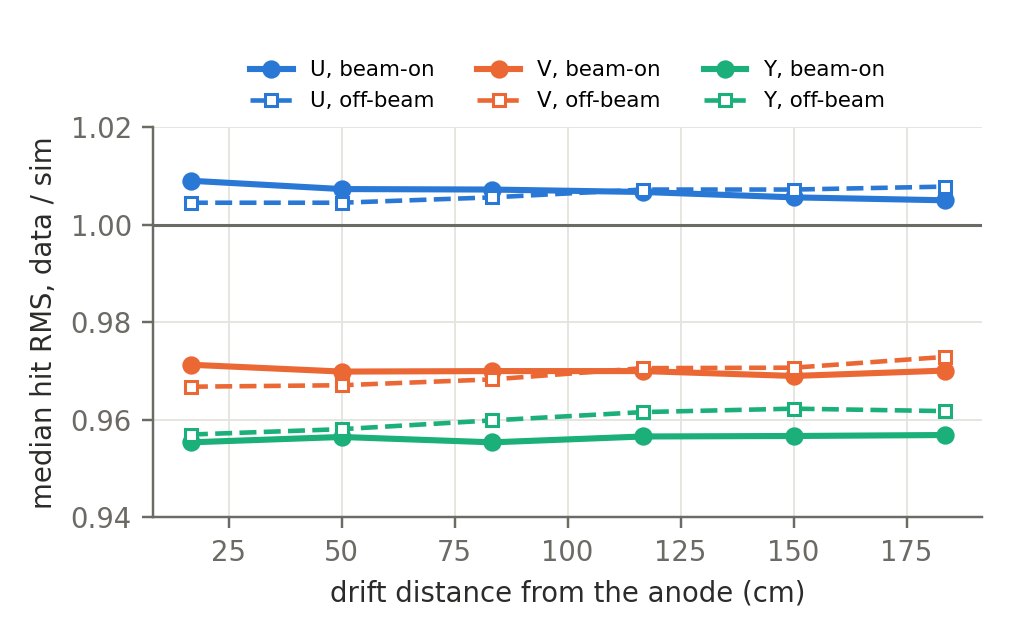
\includegraphics[width=\linewidth]{figs/width_ratio.png}
    \end{column}
    \begin{column}{0.42\textwidth}
      \footnotesize
      \begin{itemize}\setlength{\itemsep}{4pt}
        \item Median hit RMS in six drift bins, all hits.
        \item \textbf{U matches; V is 3\% and Y 4.5\% narrower in data}, the same in beam-on and off-beam.
        \item \textbf{Flat in drift.} On MicroBooNE the data/sim factor falls with drift (a diffusion mismatch, Sunny's
          measurement, \iss{9}). A constant per-plane offset points to the field response or the shaping, not diffusion.
        \item Caveat: medians over all hits, not a track-matched measurement like \iss{9}.
        \item Width was qlfm's main data/simulation cue on MicroBooNE.
      \end{itemize}
    \end{column}
  \end{columns}
\end{frame}

\begin{frame}{E3: light timing}
  \begin{columns}[T]
    \begin{column}{0.56\textwidth}
      \centering
      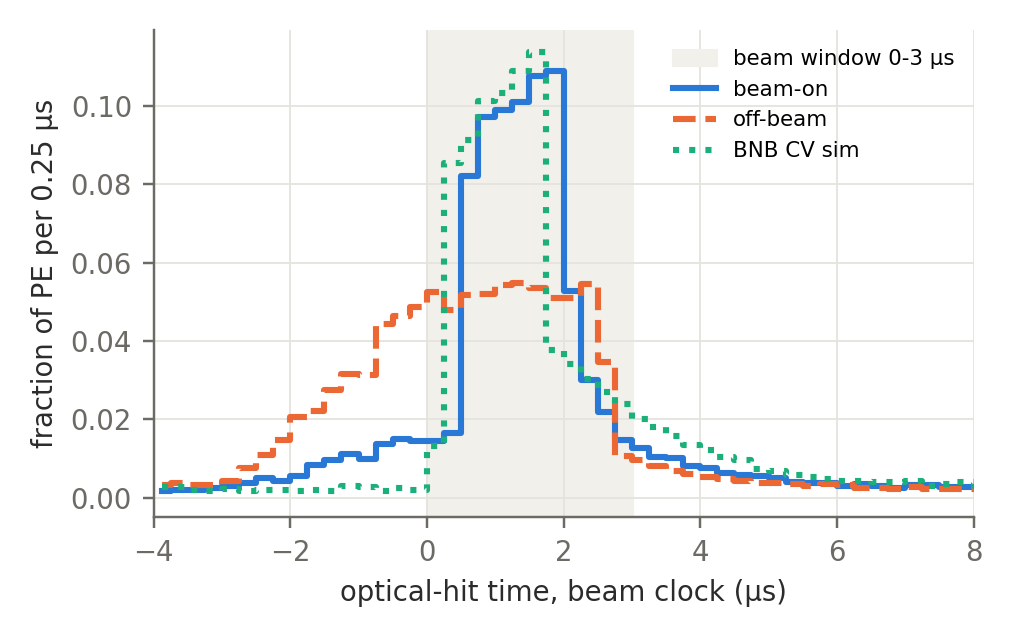
\includegraphics[width=\linewidth]{figs/light_profile.png}
    \end{column}
    \begin{column}{0.42\textwidth}
      \footnotesize
      \begin{itemize}\setlength{\itemsep}{4pt}
        \item PE-weighted optical-hit time on the beam clock, normalised per sample.
        \item \textbf{Beam-on light is $\approx$0.3\,$\mu$s later than simulation} (brightest-flash median 1.28 vs 0.99\,$\mu$s).
          Small against the 3\,$\mu$s window, but a model can read it.
        \item \textbf{Off-beam light is spread over $-3\ldots3\,\mu$s}: a different trigger window. A third of off-beam events have
          their brightest flash outside the beam window.
        \item Flash time alone separates beam-on from off-beam with AUC 0.62. When off-beam serves as ``no $\nu$'', compare
          methods at a \textbf{fixed off-beam rate}, and check events with a beam-window flash separately.
      \end{itemize}
    \end{column}
  \end{columns}
\end{frame}

\begin{frame}{E4 setup: models and metrics}
  \footnotesize
  \begin{columns}[T]
    \begin{column}{0.54\textwidth}
      \centering
      \scriptsize
      \textbf{The 13 models} (E2; multi-task, fine-tuned on the SBND simulation with 1\% labels; simulation test)\\[3pt]
      \fitw{\begin{tabular}{lcccccc}
        \toprule
        model & seeds & T1 F1 & T2 AUC & T3 F1 & T4 res & T5 MSE \\
        \midrule
        SBND-pretrained CL, fine-tuned & 3 & 0.921 & 0.996 & 0.77 & 0.22 & 0.62 \\
        SBND-pretrained C+XF & 3 & 0.896 & 0.992 & 0.73 & 0.23 & 0.78 \\
        MicroBooNE-pretrained CL & 3 & 0.903 & 0.995 & 0.74 & 0.23 & 0.74 \\
        SBND-pretrained CL, frozen & 1 & 0.876 & 0.997 & 0.72 & 0.23 & 0.59 \\
        no pretraining & 3 & 0.804 & 0.995 & 0.68 & 0.25 & 0.94 \\
        \bottomrule
      \end{tabular}}\\[3pt]
      {\tiny CL = qlfm-M with light in pretraining; C+XF = charge-only pretraining, light fused at the head.
      T1 hits, T2 $\nu$/no-$\nu$, T3 flavour, T4 energy, T5 light from charge.}
    \end{column}
    \begin{column}{0.44\textwidth}
      \begin{itemize}\setlength{\itemsep}{3pt}
        \item \textbf{Run on every event} of both samples, no retraining (0.4 node-h, debug queue).
        \item \textbf{Event level:} each model's $\nu$ log-odds cut is set so it passes the \emph{same off-beam fraction} as Wire-Cell;
          compare beam-on pass rates.
        \item \textbf{Hit level}, on beam-on events with a Wire-Cell candidate (40,404):
          \begin{itemize}
            \item share of Wire-Cell's $\nu$ charge the model also tags;
            \item share of the model's $\nu$ charge inside the Wire-Cell footprint.
          \end{itemize}
        \item \textbf{Reference:} the same hit shares on each model's simulation test split (9,368 events with a candidate).
      \end{itemize}
    \end{column}
  \end{columns}
\end{frame}

\begin{frame}{E4: event level}
  \begin{columns}[T]
    \begin{column}{0.52\textwidth}
      \centering
      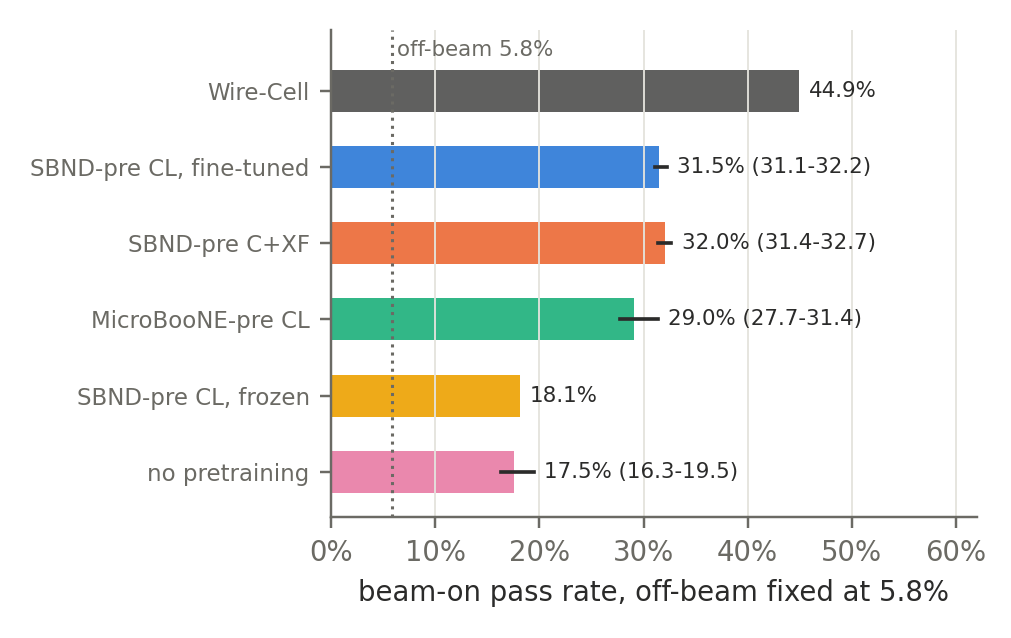
\includegraphics[width=\linewidth]{figs/event_level.png}
    \end{column}
    \begin{column}{0.46\textwidth}
      \centering
      \scriptsize
      beam-on pass rate at Wire-Cell's off-beam rate\\[3pt]
      \fitw{\begin{tabular}{lccc}
        \toprule
        & \code{wc}, all & \code{wc}, flash in window & \code{wc0} \\
        off-beam fixed at & 5.8\% & 8.4\% & 3.2\% \\
        \midrule
        \textbf{Wire-Cell} & \textbf{44.9\%} & \textbf{48.4\%} & \textbf{38.6\%} \\
        SBND-pre CL & 31.1--32.2 & 34.2--35.6 & 25.8--26.9 \\
        SBND-pre C+XF & 31.4--32.7 & 35.2--36.0 & 26.2--27.3 \\
        MicroBooNE-pre CL & 27.7--31.4 & 30.0--34.4 & 20.2--24.6 \\
        SBND-pre CL, frozen & 18.1 & 20.0 & 12.6 \\
        no pretraining & 16.3--19.5 & 18.6--22.6 & 11.1--13.5 \\
        \bottomrule
      \end{tabular}}\\[4pt]
      \raggedright\footnotesize
      \begin{itemize}\setlength{\itemsep}{2pt}
        \item SBND-pretrained fine-tuned models keep \textbf{about 2/3 of Wire-Cell's beam-on excess} over off-beam (25--27 vs 39 points); MicroBooNE-pretrained 22--26.
        \item The ordering holds with the beam-window restriction and with the cosmic-tagged label.
      \end{itemize}
    \end{column}
  \end{columns}
\end{frame}

\begin{frame}{E4: hit level}
  \begin{columns}[T]
    \begin{column}{0.56\textwidth}
      \centering
      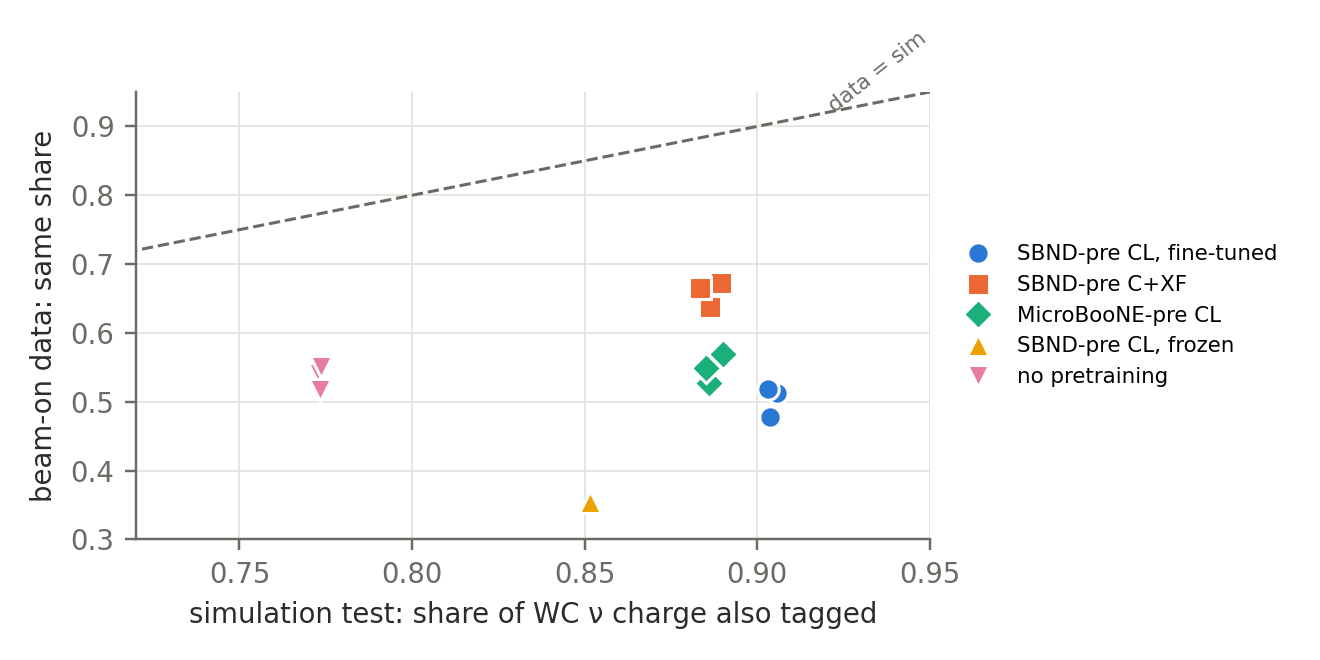
\includegraphics[width=\linewidth]{figs/agreement.png}\\[2pt]
      \scriptsize
      \fitw{\begin{tabular}{lccc}
        \toprule
        & model charge in WC footprint & \multicolumn{2}{c}{share of all charge called $\nu$} \\
        & data / sim & beam-on & off-beam \\
        \midrule
        Wire-Cell & -- & 3.8\% & 0.49\% \\
        SBND-pre CL & 0.84--0.86 / 0.90 & 2.8--3.2\% & 0.9--1.1\% \\
        SBND-pre C+XF & 0.82--0.83 / 0.88 & 4.1--4.6\% & 2.1--2.9\% \\
        MicroBooNE-pre CL & 0.80--0.82 / 0.89 & 3.4--3.8\% & 1.5--2.0\% \\
        no pretraining & 0.71--0.72 / 0.82 & 4.1--4.4\% & 3.0--3.1\% \\
        \bottomrule
      \end{tabular}}
    \end{column}
    \begin{column}{0.42\textwidth}
      \footnotesize
      \begin{itemize}\setlength{\itemsep}{4pt}
        \item \textbf{Every model falls well below the diagonal:} 0.77--0.91 of Wire-Cell's $\nu$ charge on simulation, 0.35--0.67 on beam-on.
        \item \textbf{They lose real $\nu$ hits rather than tag cosmics:} what they tag is still mostly inside Wire-Cell's footprint.
        \item \textbf{C+XF keeps the most} on data (0.64--0.67 vs 0.48--0.52 for CL), but calls more off-beam charge $\nu$.
        \item The best model on simulation (SBND-pre CL) drops the most among the fine-tuned ones; the frozen backbone drops further (0.35).
        \item The cosmic-tagged label \code{wc0} gives the same picture (shares +0.01--0.02).
      \end{itemize}
    \end{column}
  \end{columns}
\end{frame}

\begin{frame}{Reading}
  \footnotesize
  \begin{enumerate}\setlength{\itemsep}{6pt}
    \item \textbf{The simulation-to-data gap seen on MicroBooNE is present on SBND.} Models trained on simulation agree with Wire-Cell at
      about 0.9 on simulation and at 0.5--0.65 on real beam-on data.
    \item \textbf{Events survive better than hits.} The SBND-pretrained fine-tuned models still select about two-thirds of Wire-Cell's
      beam-on excess at the same off-beam rate.
    \item \textbf{Pretraining matters on data too.} Fine-tuned pretrained models (SBND or MicroBooNE) beat the frozen and the
      no-pretraining models at event level by more than a factor 1.5.
    \item \textbf{A width cue is the leading suspect, not yet tested.} On MicroBooNE the drop followed each model's reliance on hit
      width, and light-in-pretraining CL relied on it most. Here CL drops more than C+XF, and the first look shows a constant
      per-plane width offset. The SBND offset is simpler than MicroBooNE's (no drift dependence), so it may be easier to correct.
  \end{enumerate}
\end{frame}

\begin{frame}{Caveats}
  \footnotesize
  \begin{itemize}\setlength{\itemsep}{5pt}
    \item \textbf{Wire-Cell is a reference, not truth, on data.} Disagreement can be the model's or Wire-Cell's; on simulation
      Wire-Cell's label has efficiency 0.92 and purity 0.95.
    \item \textbf{No exposure normalisation.} Off-beam has no spill count here; comparisons are pass rates at a matched off-beam
      rate, not $\nu$ rates per POT.
    \item \textbf{Trigger selection.} Both data samples are light-triggered; the simulation is not. The simulation reference is on
      unselected events with a $\nu$; this does not change the size of the drop.
    \item \textbf{Off-beam light timing differs} from beam-on; handled only by the beam-window restriction.
    \item \textbf{Hit producer settings in data not verified} beyond the \code{gaushit} label.
    \item \textbf{First-look widths are medians over all hits}, mostly cosmics, not a track-matched measurement.
  \end{itemize}
\end{frame}

\begin{frame}{Next steps (proposed, not started)}
  \footnotesize
  \begin{enumerate}\setlength{\itemsep}{6pt}
    \item \textbf{Width test on SBND simulation:} rescale simulated V and Y hit widths by the measured 0.97 / 0.955 at test time. Does
      the simulation agreement fall to the data level? Same procedure as \iss{9}.
    \item \textbf{Width-randomised or width-free fine-tune} on the SBND simulation, then rerun E4.
    \item \textbf{Light-trigger emulation in the simulation} (beam-window PE threshold matched to the data turn-on), so simulation
      and data rates are comparable.
    \item \textbf{Event displays} of beam-on events where Wire-Cell and the models disagree.
    \item \textbf{Track-matched width and charge comparison} on SBND cosmics (as Sunny did for MicroBooNE), and the data GausHit
      FHiCL.
  \end{enumerate}
\end{frame}

%=====================================================================
\begin{frame}{Backup: where everything is}
  \scriptsize
  \begin{itemize}\setlength{\itemsep}{3pt}
    \item \textbf{Issue log:} \iss{14} (production, first look, E4, trigger note), \iss{11} (simulation samples, label fix).
    \item \textbf{Docs:} \doc{sbnd-realdata.md} (recipe, label definition), \doc{sbnd-h5maker.md} (simulation sample),
      \doc{data-inventory-sbnd.md}, \doc{experiments-live.pdf} (status board).
    \item \textbf{Data:} \code{fm4npp-lartpc-data/sbnd-data-\{bnb-opendata,offbeam-intime-run1\}/} (\code{full/}, \code{lists/}, README with POT and upstream selection).
    \item \textbf{Caches:} \code{\$QLFM\_WORK/cache/sbnd\_data\_m/} (data), \code{cache/sbnd\_m/} (simulation).
    \item \textbf{Results:} \code{\$QLFM\_WORK/sbnd\_data/firstlook.json}; \code{sbnd\_data/eval/<run>/report.json}, all runs in \code{report\_all.jsonl}.
    \item \textbf{Code} (fm4npp-lartpc main): converter data mode 5af5e9a; first look eb29862; \code{eval\_sbnd\_data} 548de25;
      \code{load\_run} fix 6987c12; \code{sbnd-h5maker} 0.5 (\code{6d03818}), FermiGrid scripts (\code{c863a07}, \code{1f6c1a7}).
    \item \textbf{Compute:} FermiGrid 37.5 CPU-h (production); Polaris about 0.5 node-h on \code{LArTPC\_FM} (conversion 0.03, smoke tests, E4 0.4).
  \end{itemize}
\end{frame}

\end{document}
